% !TEX root = main.tex
\begin{figure} 
    \centering
  \subfloat[\label{1a}]{%
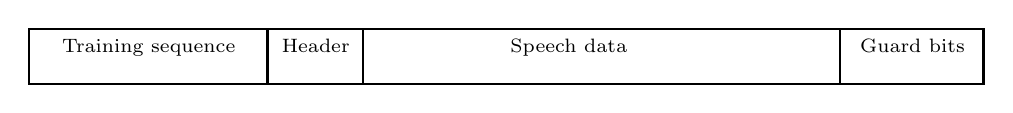
\begin{tikzpicture}[                
                    slot/.style={
            		text centered,
			font=\scriptsize,
			align=center,
			anchor=center,
			minimum height=0.7cm
            	}]
\draw[thick] (0,0) rectangle (\linewidth, -0.7);
\draw[thick] (0.25\linewidth,0) -- ++(0, -0.7);
\draw[thick] (0.35\linewidth,0) -- ++(0, -0.7);
\draw[thick] (0.85\linewidth,0) -- ++(0, -0.7);

\draw
(0,0) node[slot, minimum width=0.25\linewidth, anchor=north west](barker){Training sequence \\ \barkerBitsQPSK}
(0.25\linewidth,0)  node[slot, minimum width=0.1\linewidth, anchor=north west](barker){Header \\ \headerBits}
(0.35\linewidth,0) node[slot, minimum width=0.43\linewidth, anchor=north west](barker){Speech data \\ \packetDataBitsQPSK}
(0.85\linewidth,0) node[slot, minimum width=0.15\linewidth, anchor=north west](barker){Guard bits \\ \guardBitsQPSK}
;	

\end{tikzpicture}
}
  \\
  \subfloat[\label{1b}]{%
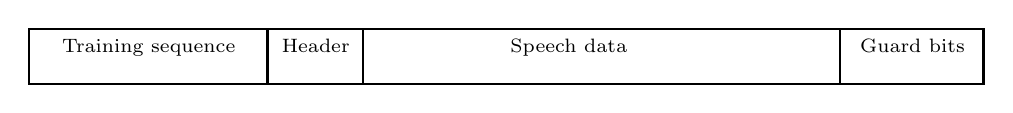
\begin{tikzpicture}[                
                    slot/.style={
            		text centered,
			font=\scriptsize,
			align=center,
			anchor=center,
			minimum height=0.7cm
            	}]
\draw[thick] (0,0) rectangle (\linewidth, -0.7);
\draw[thick] (0.25\linewidth,0) -- ++(0, -0.7);
\draw[thick] (0.35\linewidth,0) -- ++(0, -0.7);
\draw[thick] (0.85\linewidth,0) -- ++(0, -0.7);

\draw
(0,0) node[slot, minimum width=0.25\linewidth, anchor=north west](barker){Training sequence \\ \barkerBitsQAM}
(0.25\linewidth,0)  node[slot, minimum width=0.1\linewidth, anchor=north west](barker){Header \\ \headerBits}
(0.35\linewidth,0) node[slot, minimum width=0.43\linewidth, anchor=north west](barker){Speech data \\ \packetDataBitsQAM}
(0.85\linewidth,0) node[slot, minimum width=0.15\linewidth, anchor=north west](barker){Guard bits \\ \guardBitsQAM}
;	

\end{tikzpicture}}
  \caption{Burst format for QPSK (a) and QAM-64 (b) modulation}
  \label{fig1} 
\end{figure}